\chapter{Array}
\section{Two-pointer Algorithm}
\runinhead{Container With Most Water.} Given coordinate $(i, a_i)$, find two lines, which together with x-axis forms a container, such that the container contains the most water.
\begin{figure}[hbtp]
\centering
\subfloat{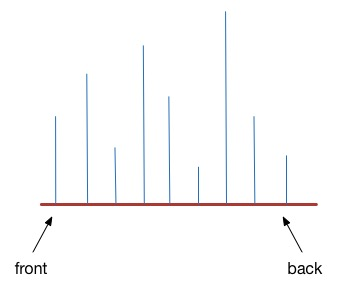
\includegraphics[scale=.50]{Container-With-Most-Water.jpg}}
\caption{Container with Most Water}
\label{fig:Container-With-Most-Water}
\end{figure}
Core clues:
\begin{enumerate}
\item \textbf{Two pointers}: $start$, $back$ at two ends. Calculate the current area
\item \textbf{Move one}: Move the shorter (lower height) pointer. 
\end{enumerate}

\section{Circular Array}
This section describes common patterns for solving problems with circular arrays.

Normally, we should solve the linear problem and circular problem differently.

\subsection{Circular max sum}
Linear problem can be solved linear with dp algorithm for maximum subarray sum - Section \ref{dpSequence}. 

The circular sum should use dp. 

Problem description: Given an integer array, find a continuous rotate subarray where the sum of numbers is the biggest. Return the index of the first number and the index of the last number. 
\runinhead{Core clues:}
\begin{enumerate}
\item \textbf{State definitions}: 

Construct left max sum $L_i$ for max sum over the $[0..i]$ with subarray starting at 0 (\textit{forward} starting from the left side). 

Construct right max sum $R_i$ for max sum over the indexes $[i+1..n -1]$, with subarray ending at -1 (\textit{backward} starting from the right side). 

Notice, for the two max sums, the index ends AT or BEFORE $i$.

\item \textbf{Transition functions:}
\begin{align*}
L_i = \max\Big(L_{i-1}, sum(A[:i])\Big) \\ 
R_i = \max\Big(R_{i+1}, sum(A[i:])\Big)
\end{align*}

\item \textbf{Global result}: 
$$maxa = \max(R_i+L_{i-1}, \forall i)$$
\end{enumerate}

\subsection{Non-adjacent cell}
Maximum sum of non-adjacent cells in an array $A$.

To solve circular non-adjacent array problem in linear way, we should consider 2 cases:
\begin{enumerate}
\item Not consider the $A[1]$
\item Not consider the $A[-1]$ 
\end{enumerate}
and solve them using linear maximum sum of non-adjacent cells separately  - Section \ref{dpSequence}. 
\subsection{Binary search}
Searching for an element in a circular sorted array. Half of the array is sorted while the other half is not.
\begin{enumerate}
\item If $A[0] < A[mid]$, then all values in the first half of the array are sorted.
\item If $A[mid] < A[-1]$, then all values in the second half of the array are sorted.
\item Then \textit{derive and decide} whether to got the \textbf{sorted half} or the \textbf{unsorted half}.
\end{enumerate}
\section{Voting Algorithm}
\subsection{Majority Number}
\subsubsection{$\frac{1}{2}$ of the Size}
Given an array of integers, the majority number is the number that occurs more than half of the size of the array. 

Algorithm: Majority Vote Algorithm. Maintain a counter to count how many times the majority number appear more than any other elements before index $i$ and after re-initialization. Re-initialization happens when the counter drops to 0. 

Proof: Find majority number $x$ in $A$. Mathematically, find $x$ in array $A$ with length $n$ s.t. $cnt_x > n -cnt_x$. 

Find a \textbf{pair} $(a_i, a_j)$ in $A$, if $a_i \neq a_j$, delete both from $A$. The counter  still
holds that: $C^{A'}_x > |A'|-C^{A'}_x$. Proof, since $a_i\neq a_j$, at most 1 of them
equals $x$, then $C^{A'}_x$ decrements at most by 1, $|A'|$ decrements by 2.

To find such pair $(a_i, a_j), a_i\neq a_j$, linear time one-pass algorithm. That's
why \textit{Moore's voting algorithm} is correct.

At any time in the execution, let $A'$ be the prefix of $A$ that has been processed,
if $counter>0$, then keep track the candidate $x$'s counter, the $x$
is the majority number of $A'$.  If $counter =0$, then for $A'$ we can pair the elements
s.t. are all pairs has distinct element. Thus, it does not hold that $cnt_x>n-cnt_x$;
thus $x\in A'$. $\blacksquare$
 
Re-check: This algorithm needs to re-check the current number being counted is indeed the majority number.    

\begin{python}
def majorityElement(self, nums):
    """
    Algorithm:
    O(n lgn) sort and take the middle one
    O(n) Moore's Voting Algorithm
    """
    mjr = nums[0]
    cnt = 0
    for i, v in enumerate(nums):
        if mjr == v:
            cnt += 1
        else:
            cnt -= 1

        if cnt < 0:
            mjr = v
            cnt = 1

    return mjr

\end{python}
\subsubsection{$\frac{1}{3}$ of the Size}
Given an array of integers, the majority number is the number that occurs more than $\frac{1}{3}$ of the size of the array. This question can be generalized to be solved by $\frac{1}{k}$ case. 

\subsubsection{$\frac{1}{k}$ of the Size}
Given an array of integers and a number k, the majority number is the number that occurs more than $\frac{1}{k}$ of the size of the array. In this case, we need to generalize the solution to $\frac{1}{2}$ majority number problem.
\newpag
\begin{python}

def majorityNumber(self, nums, k):
    """
    Since majority elements appears more 
    than ceil(n/k) times, there are at 
    most k-1 majority number
    """
    cnt = defaultdict(int)
    for num in nums:
        if num in cnt:
            cnt[num] += 1
        else:
            if len(cnt) < k-1:
                cnt[num] += 1
            else:
                for key in cnt.keys():
                    cnt[key] -= 1
                    if cnt[key] == 0: del cnt[key]
    
    
    # filter, double-check
    for key in cnt.keys():
        if (len(filter(lambda x: x == key, nums)) 
            > len(nums)/k):
            return key

    raise Exception
\end{python}


\section{Two Pointers}
\subsection{Interleaving}
\runinhead{Interleaving positive and negative numbers.} Given an array with positive and negative integers. Re-range it to interleaving with positive and negative integers.
\begin{lstlisting}
Input:
[-33, -19, 30, 26, 21, -9]
Output:
[-33, 30, -19, 26, -9, 21]
\end{lstlisting}
Core clues:
\begin{enumerate}
\item In 1-pass.
\item What (positive or negative) is expected for the current position.
\item Where is the next positive and negative element.
\end{enumerate}
\begin{python}
def rerange(self, A):
    n = len(A)
    pos_cnt = len(filter(lambda x: x > 0, A))
    pos_expt = True if pos_cnt*2 > n else False

    neg = 0  # next negative
    pos = 0  # next positive
    for i in xrange(n):
        while neg < n and A[neg] > 0: neg += 1
        while pos < n and A[pos] < 0: pos += 1
        if pos_expt:
            A[i], A[pos] = A[pos], A[i]
        else:
            A[i], A[neg] = A[neg], A[i]

        if i == neg: neg += 1
        if i == pos: pos += 1

        pos_expt = not pos_expt
\end{python}

\section{Index Remapping}
\subsection{Introduction}
\runinhead{Virtual Index.} Analogy to physical machine and virtual machine, the underlying indexing $i$ for array $A$ is the physical index. We can create virtual indexing $i'$ for the same array $A$ to map $A_{i'}$ to the physical entry $A_{i}$.
\subsection{Example}
\runinhead{Interleaving indexes} Given an array $A$ of length $n$, we want to mapping the virtual indexes to physical indexes such that $A_0$ maps to $A_1$, $A_1$ maps to $A_3$,..., $A_{\lfloor n/2\rfloor}$ maps to $A_0$, as followed: 
\begin{figure}[hbtp]
\centering
\subfloat{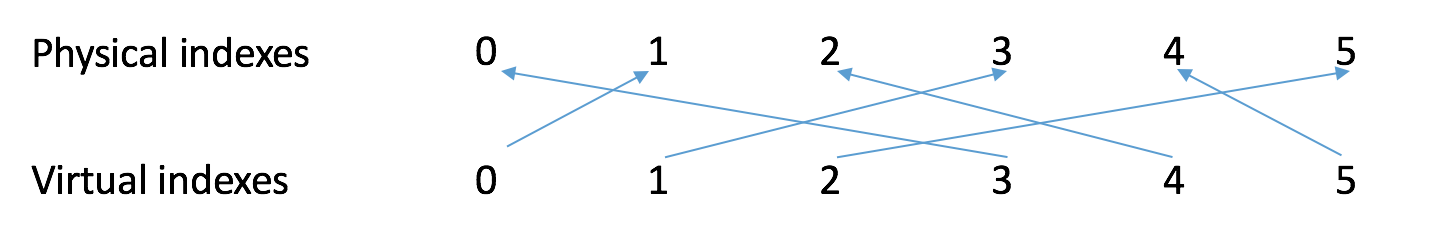
\includegraphics[scale=.70]{virtual_indexes.png}}
\caption{Virtual Indexes. Remapping}
\label{fig:virtual_indexes}
\end{figure}
\begin{lstlisting}
0 -> 1
1 -> 3
2 -> 5
...
n/2-1 -> n-1 or n-2

n/2 -> 0
n/2+1 -> 2
...
n -> n-2 or n-1
\end{lstlisting}
If $n$ is even, 
$$
(2*i+1)\%(n+1)
$$
If $n$ is odd,
$$
(2*i+1)\%(n)
$$
Thus, by combining two cases, we create the mapping relationship: 
\begin{python}
def idx(i):
    return (2*i+1) % (n|1)
\end{python}

